\chapter{Results}
%The following images show the result of mapping using handheld Kinect:

\begin{figure}[ht]
	\begin{center}
		
		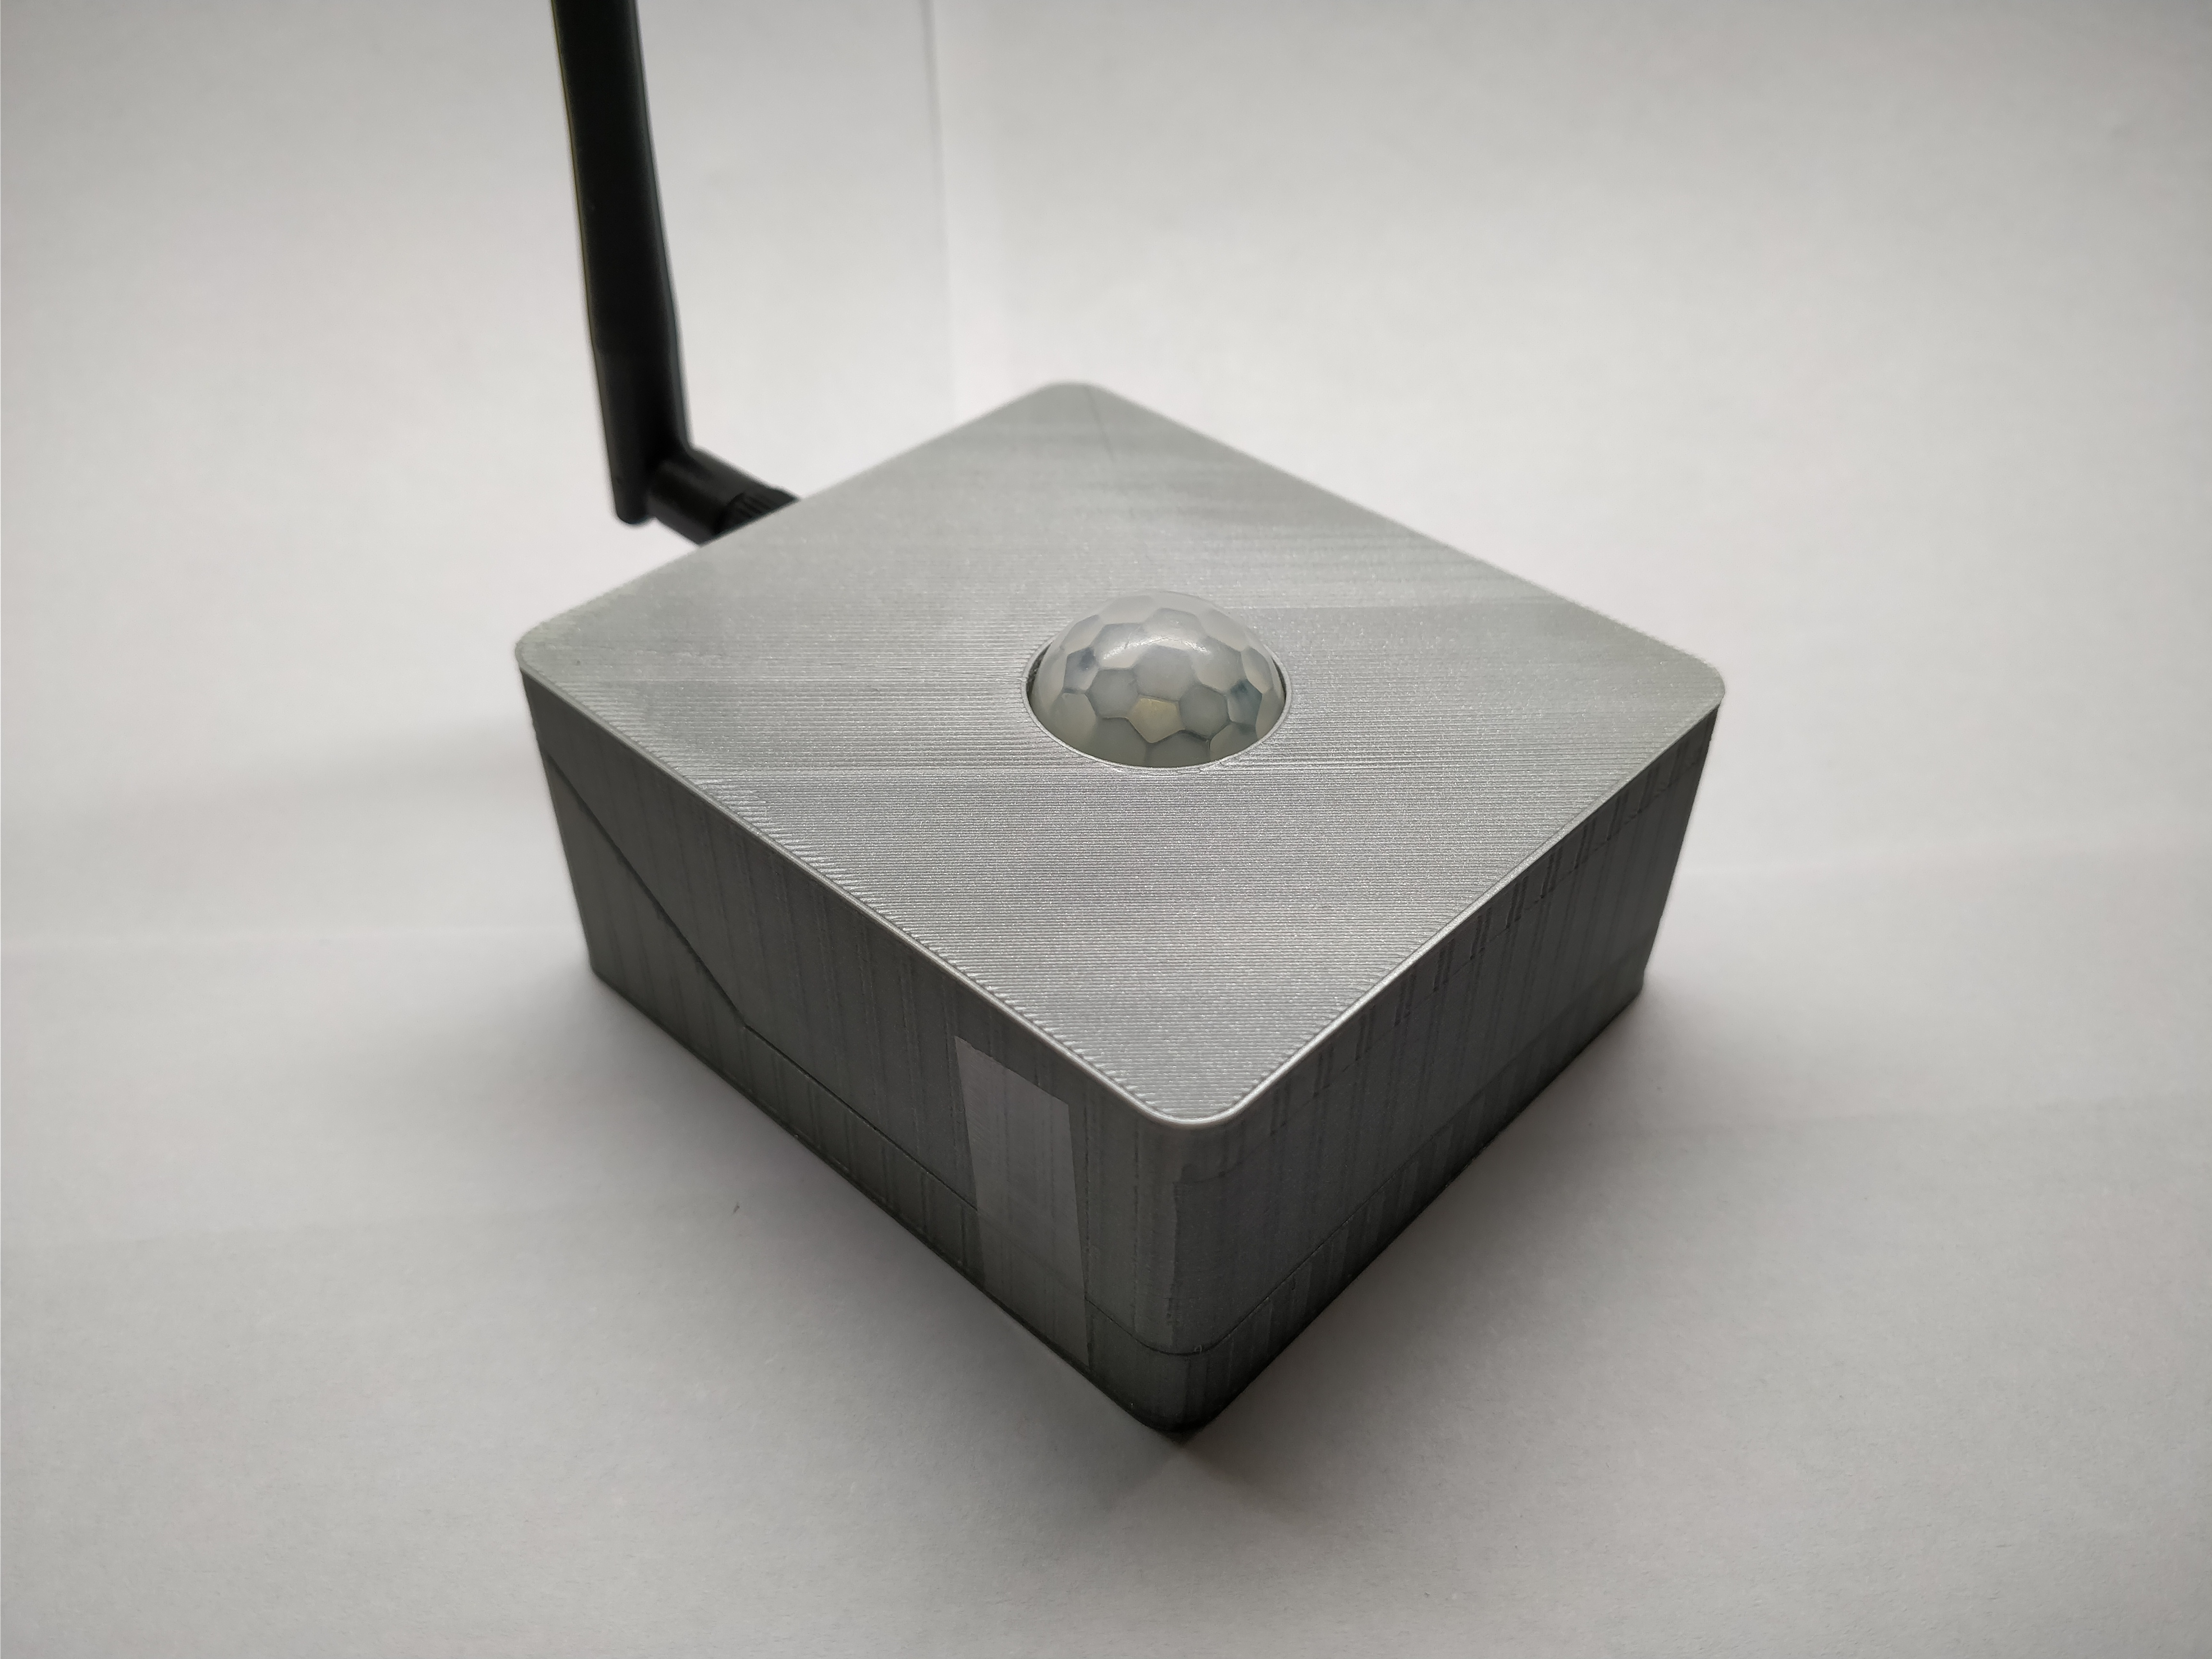
\includegraphics[scale=.075]{FinalProduct.jpg}
		
		\caption{Final Assembled Device}
		%\label{fig:Final}
		
		\end{center}
\end{figure}

The devices have been configured in a tree network setup. All the end nodes stay in a deep sleep state. They wake up only when a change of state in the PIR sensor is detected or when the WDT overflows. 

When motion is detected the device wakes up from its deep sleep state using interrupts and then transmits the required information and goes back to its deep sleep state. 
The devices also periodically wake up and send the state when the WDT overflows. This is so that if a device fails the master can sense that the device hasn't transmitted anything recently and then that device can be marked offline by the user.

The routers are always awake and listening so that they can route information between the devices and the master whenever required. They can be battery powered or can be powered using a mains adapter.

\begin{center}
	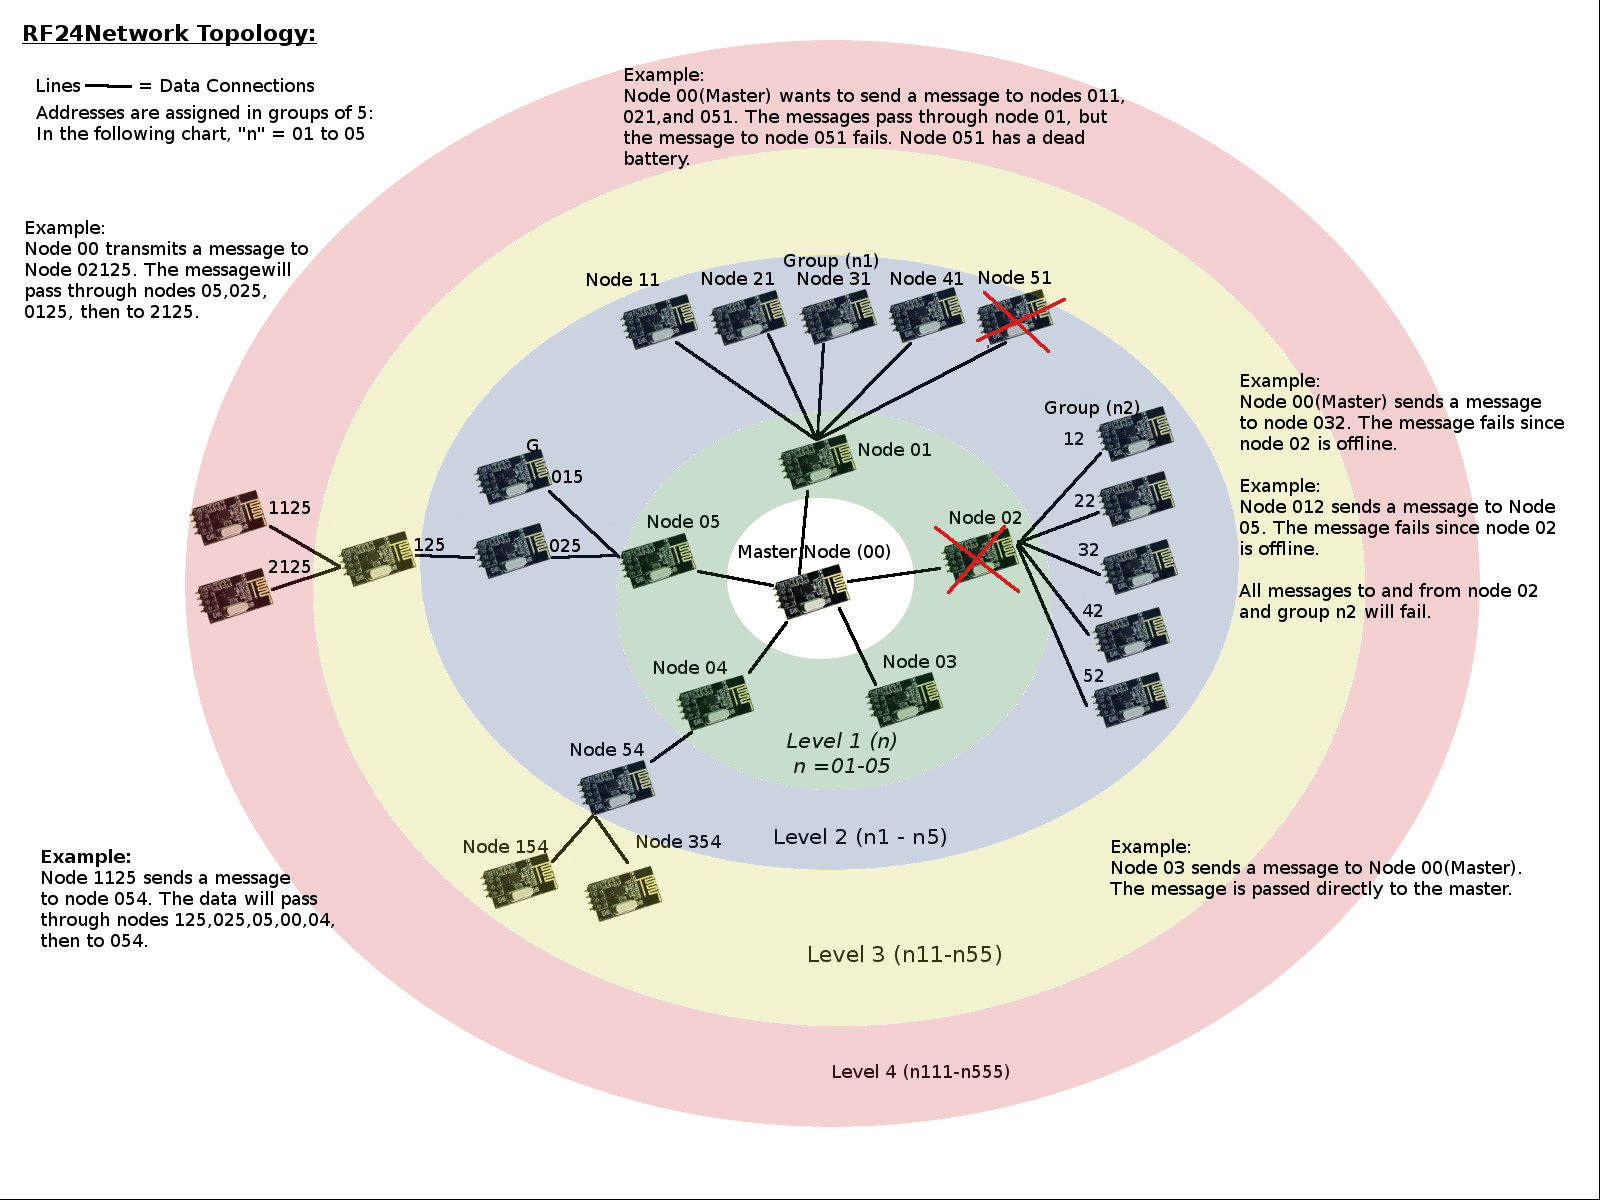
\includegraphics[scale=.17]{TreeNW.jpg}
	
	Tree network topology
\end{center}

\begin{center}
	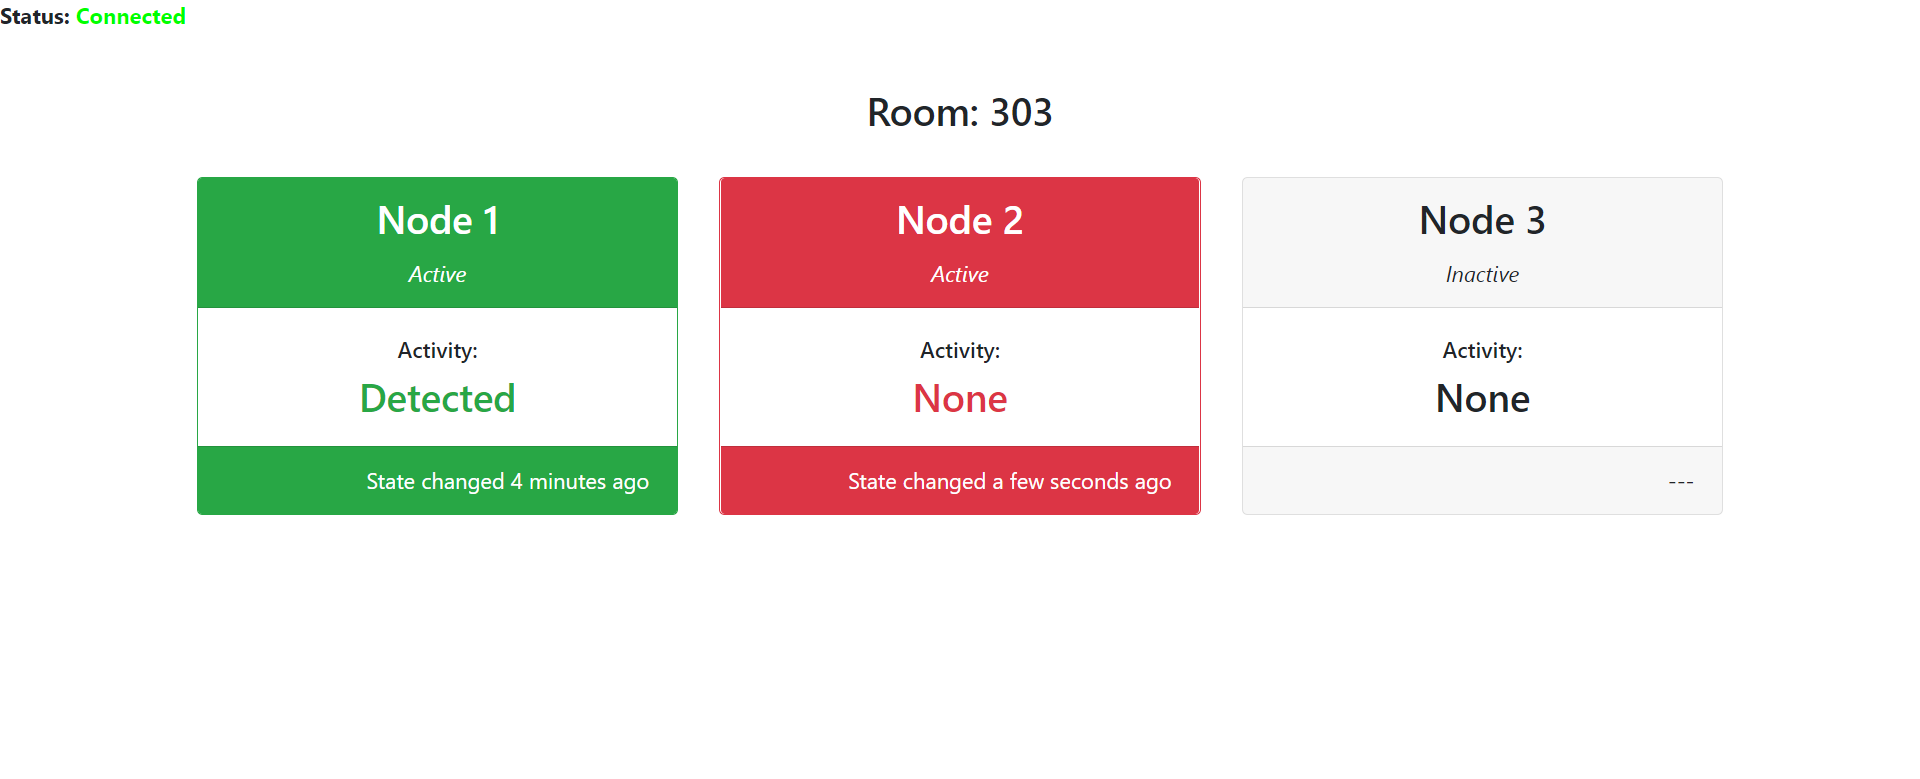
\includegraphics[scale=0.25]{Website1.png}
	\\Website
\end{center}

Real time occupancy status can be seen 


